In examining the influence of $\alpha$ on the roots of the equation 6 ($\alpha - x^2$) and equation 7 ($\alpha - 2x^3 - 3$), we implemented the function \texttt{plot\_bifurcation\_diagram}. This function begins by generating an $\alpha$ spectrum based on specified initial and endpoints, along with the desired number of data points, utilizing \texttt{numpy}'s \texttt{linspace} function.

Subsequently, within the for loop iterating over \texttt{alpha\_values}, the functions \texttt{equation6} and \texttt{equation7} come into play. The return values of these functions are systematically filled with corresponding $\alpha$ values. Leveraging \texttt{numpy}'s \texttt{roots} method, we ascertain the roots of the polynomial list derived from these functions.

The resultant root values are then employed to construct a comprehensive graph. Here, the x-axis delineates $\alpha$ values, while the y-axis represents the corresponding Steady States' values. For a visual representation, refer to Figure \ref{fig:task2}.

To enhance the interpretability of the graph in terms of stability, we introduced distinctive blue and red points along the x-axis. Blue points indicate the presence of roots, signaling stability in the system. Conversely, red points highlight the absence of roots, pointing towards instability for the associated $\alpha$ values in equations 6 and 7. This visual aid provides a clear delineation of stability patterns across the parameter space.


\begin{figure}[H]
    \centering
    \begin{subfigure}[b]{0.45\textwidth}
        \centering
        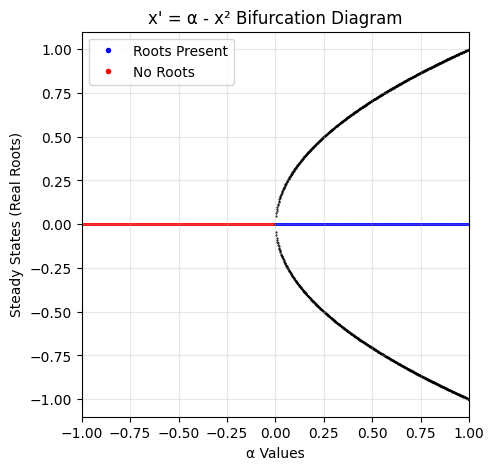
\includegraphics[width=\textwidth]{images/task2eq6.png}
        \label{fig:subfig1}
    \end{subfigure}
    \hfill
    \begin{subfigure}[b]{0.45\textwidth}
        \centering
        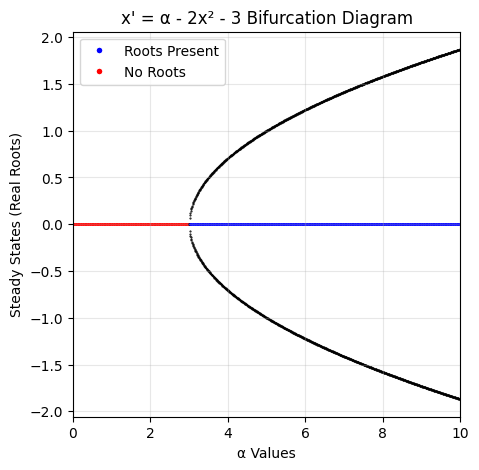
\includegraphics[width=\textwidth]{images/task2eq7.png}
        \label{fig:subfig2}
    \end{subfigure}
    \caption{Bifurcation Diagrams of $x' = \alpha - x^2$ and $x' = \alpha - 2x^2 - 3$}
    \label{fig:task2}
\end{figure}


In examining equation 7, the initial threshold range of -1 to 1 proved insufficient, prompting an extension of the interval to 0 to 10 for a more comprehensive investigation. The analysis involved a total of 1001 points for both equations 6 and 7, ranging from +1 to 1000. This broad range was purposely chosen to gain a thorough understanding of the system's behavior, with a specific focus on the pivotal middle point (0) of the steady state.

Concerning equation 6, a key observation is that points greater than 0 consistently yield two real roots. Conversely, for points smaller than 0, real roots are not feasible due to the inherent impossibility of a square of a real number being equal to a negative value in real systems.

Taking a deeper dive into the analysis, at the critical 0 point, a \textbf{saddle-node bifurcation} occurs. This intriguing phenomenon signifies the collision and subsequent annihilation of two fixed points within the dynamical system. The manifestation is visually depicted by a small black point, acting as a clear separator between the blue and red lines on the graph, with a singular root located at (0,0).

Additionally, it's noteworthy that the density of points around 0 is noticeably reduced. This phenomenon can be attributed to the heightened sensitivity of root values to slight variations in $\alpha$. The system undergoes rapid and significant alterations in the root values with minor changes in $\alpha$, resulting in an elongated $\alpha$ interval around the zero point. This observation underscores the intricate dynamics of the system, highlighting its responsiveness to subtle fluctuations in parameter values. \\

Observing the bifurcation diagram for equation 7 reveals a parallel occurrence to equation 6, albeit in distinct regions. Notably, for equation 7, the point density diminishes as we approach $\alpha=3$. No points exist for $\alpha$ values smaller than 3, while there are consistently two points for values greater than 3. The bifurcation type observed in this scenario is also identified as a \textbf{saddle-node bifurcation}. \\

Beyond the visual similarity in the diagrams, a more explicit connection between equation 6 and equation 7 can be established. Both equations are 2nd-order polynomials, with equation 7 exhibiting a 3-unit delay to the right and a narrower profile due to the coefficient of 2 for $x^2$. This relationship allows us to explicitly demonstrate that equation 6 can be mapped to equation 7 (or vice versa) through a combination of delay and multiplication. Consequently, we can assert that these two equations share the \textbf{same normal form}.

The \textbf{topological equivalence} of these two equations is notable at the point $\alpha = -1$, where both equations share the absence of steady states, placing them in the same dynamical situation. However, this equivalence breaks down at $\alpha = 1$. At this juncture, equation 6 features 2 steady states, while equation 7 continues to lack any steady states. This distinction highlights the sensitivity of the system's behavior to changes in the parameter $\alpha$, leading to divergent dynamics at different values of $\alpha$.